\documentclass[/home/greg/Thesis/main/main.tex]{subfiles}

\begin{document}
\graphicspath{{/home/greg/Neutron_star_modelling/MotionOfARigidBody/img}}
\newcommand{\MotionOfARigidBodyDir}{/home/greg/Neutron_star_modelling/MotionOfARigidBody}

\newcommand{\dn}{\mathrm{dn}}

\FloatBarrier
As \citet{Landau1969} described, the motion of $\mathbf{M}$ in the rotating frame
can be understood by the use of conservation laws. For the time being let us consider,
in the rotating frame, a torque free body with moments of inertia $I_{1}, I_{2}, I_{3}$. 
If the spin-vector components are given by $M_{i} = I_{i} \Omega_{i}$ then 
in momentum space, we can write the conservation of energy and angular momentum as
\begin{align}
    \frac{M_{1}^{2}}{I_{1}} + \frac{M_{2}^{2}}{I_{2}} + \frac{M_{3}^{2}}{I_{3}} = 2E 
    \label{eqn: ellipse} \\
    M_{1}^{2} + M_{2}^{2} + M_{3}^{2} = M^{2}
    \label{eqn: sphere}
\end{align}
The conservation of energy describes an ellipsoid with semi-axis
$\sqrt{2EI_{1}}, \sqrt{2EI_{2}}$ and $\sqrt{2EI_{3}}$. The conservation of 
angular momentum describes a sphere of radius $M$. The intersection of the
sphere and ellipse at fixed $E$ and $M$ describe the precession of the angular
momentum and hence the spin-vector.

\section{Torque free biaxial body}
For a biaxial body free from torques we can parameterise the principle components
of the moment of inertia by 
\begin{align}
    I_{1} = I_{2} = I_{0}, &&& I_{3} = I_{0}(1 + \epsI)
\end{align}
For such a system, the Euler rigid body equations have an
exact solution with $\Omega_{3}=$ const. and the other components are given by
\begin{align}
    \Omega_{1} &= A\cos\left(\epsI \Omega_{3} t\right),\\
    \Omega_{2} &= A\sin\left(\epsI \Omega_{3} t\right),
\end{align}
where the constant can be written as
\begin{align}
    A & = \left(\Omega^{2} - \Omega_{3}^{2}\right)^{1/2}\\
      & = \left(\frac{M^{2} - M_{3}^{2}}{I_{0}^{2}}\right)^{1/2}.
\end{align}
We note that $\Omega^{2}$ is also a constant, since there is no torque. In the rotating
body frame, this solution demonstrates that the spin-vector will precess in a
circle about the symmetry axis. The circle is precisely the intersection of the
ellipsoid and sphere. Since the cone is aligned with the $3$ axis, we can define
a polar angle $\theta$ made by the momentum-vector with the $3$ axis. This will be 
constant during a precessional period and can be calculated as follows:
\begin{equation}
\sin\theta = \frac{M_{3}}{M}
\label{eqn: sin theta}
\end{equation}
In the work of \citet{Jones2001}, the angle $\theta$ was referred to as the 
\emph{wobble angle} meaning the angle of precession.

\begin{figure}[htb]
\centering
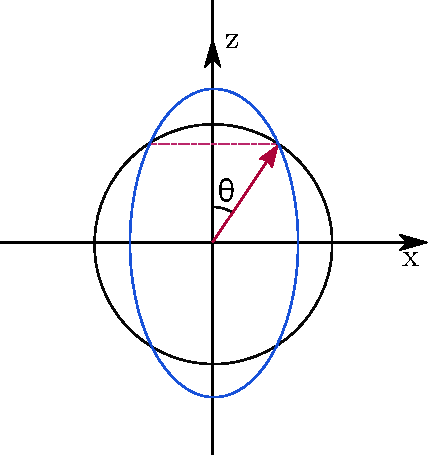
\includegraphics[width=0.4\textwidth]{\MotionOfARigidBodyDir/../Illustrations/SphereEllipse/SphereEllipseBiaxial}
\caption{A slice through the $z-x$ in momentum space showing the sphere described
by the conservation of angular momentum and ellisoid due to the conservation of
energy. Since both of these conservation laws must be satisfied, this restricts
the motion of $\mathbf{M}$ to intersection. For this biaxial body the intersection
is a circle about the $\z$ axis, as a result the momentum vector traces out a
cone of half angle~$\theta$ about this axis.}
\label{fig: sphere ellispod biaxial}
\end{figure}

To calculate the wobble angle in terms of the energy and momentum, 
from equation \eqref{eqn: ellipse} we can rearrange to get
\begin{align}
    M_{3}^{2} & = (1+\epsI)\left(2EI_{0} - M_{1}^{2} - M_{2}^{2}\right) \\
              & = (1+\epsI)\left(2EI_{0} - \left(M^{2} - M_{3}^{2}\right)\right)
\end{align}
Expanding and solving for $M_{3}^{2}/M^{2}$ 
\begin{align}
    \frac{M_{3}^{2}}{M^{2}} = \frac{1+\epsI}{\epsI}\left(1 - \frac{2EI_{0}}{M^{2}}\right)
\end{align}
Then we can write the polar angle as
\begin{equation}
    \sin\theta = \left(\frac{1+\epsI}{\epsI}\left(1 - \frac{2EI_{0}}{M^{2}}\right)\right)^{1/2}
    \label{eqn: sin theta biaxial}
\end{equation}
The term in brackets contains the ratio of the square of smallest semi-axis of
the ellisoid and the radius of the sphere. That is
\begin{align}
    \frac{2EI_{0}}{M^{2}} = \left(\frac{\sqrt{2EI_{0}}}{M}\right)^{2}
\end{align}
This provides an intuitive way to think about the wobble angle: as the smallest
semi-axis of the ellipse approaches the radius of the sphere $\sqrt{2EI_{0}}\rightarrow M$
then $\theta$ tends to zero. That is, the circles of intersection between the
sphere and ellipse close up around the $z$ axis.

\section{Torque free triaxial body}
Let us now consider the case of a triaxial body with moments of inertia in the
body frame satisifying
\begin{equation}
    I_{1} < I_{2} < I_{3}
\end{equation}
As described by the \citet{Landau1969} the motion of $\mathbf{M}$ is
described by the intersection of the sphere and now triaxial ellipsoid
with semiaxis $\sqrt{2EI_{1}}, \sqrt{2EI_{2}}$ and $\sqrt{2EI_{3}}$. These 
intersection are complicated but a sketch is provided in figure 51 of 
\citet{Landau1969}.

% Add description - copy from elsewhere?

Solutions to the components of $\Omega_{i}$ in the rotating frame are given 
by \citet{Landau1969} in terms of Jacobian elliptic functions. For definiteness
the suppose that $M^{2} > 2EI_{2}$ such that the momentum precesses about the
$\z$ axis. If this inequality is reversed then the momentum will precess
about the $\x$ axis. As such as should therefore define the angle $\theta$ 
by replacing 3 with 1 in equation \eqref{eqn: sin theta}; if this were the case
we would swap the $1$ and $3$ suffixes in the following formulae.

Continuing with precession about the $\z$ axis, we have that
\begin{equation}
    \Omega_{3} = \sqrt{\frac{M^{2} - 2EI_{1}}{I_{3}\left(I_{3} - I_{1}\right)}} 
                 \dn(\tau , k^{2}).
\end{equation}
where $\dn(\tau, k^{2})$ is an elliptic function, with the dimensionless time variable
$\tau$ given by 
\begin{equation}
    \tau = t\sqrt{(\frac{I_{3} - I_{2})(M^{2} - 2EI_{1})}{I_{1}I_{2}I_{3}}}
    \label{eqn: tau t}
\end{equation}
and the elliptic parameter $k^{2}$ is bounded by $[0, 1]$ and given by 
\begin{equation}
    k^{2} = \frac{(I_{2} - I_{1})(2EI_{3} - M^{2})}{(I_{3}-I_{2})(M^{2} - 2EI_{1})}
    \label{eqn: k2}
\end{equation}
The polar angle in the triaxial case can then be written
\begin{align}
    \sin\theta & = \frac{M_{3}}{M} \\
               & = \frac{I_{3}\Omega_{3}}{M} \\
               & = \sqrt{\frac{I_{3}(1 - 2EI_{1}/M^{2})}{\left(I_{3} - I_{1}\right)}} 
                   \dn(\tau, k^{2})
\end{align}
The coefficients of the elliptic integral is constructed from constants, so only
the elliptic function $\dn(\tau, k^{2})$ contributes to the time dependance of the
polar angle. 

The variable $k$ measures the `triaxiality' of the body: in the limit 
$k\rightarrow 0$ when the body becomes biaxial, $dn(\tau, k) \rightarrow 1$. 
That is, in the biaxial limit $\Omega_{3}$ tends to a constant such that
$\sin\theta$ tends to the constant given in equation\eqref{eqn: sin theta biaxial}.

\subsubsection{Aside on the elliptic function}
We now briefly review the features of the elliptic function $\dn(\tau, k)$. 
Firstly we note that there an alternaive convention used by \citet{Abramowitz1972}
in which $m := k^{2}$; the elliptic function is then written $\dn(\tau| m)$. 

$\dn(\tau, k)$ is a periodic function: in $\tau$ the period is $4K$ where 
$K$ is a complete elliptic integral of the first kind:
\begin{align}
    K(k) = \int_{0}^{\pi/2}\frac{d\tau}{\sqrt{1 - k^{2}\sin^{2}\tau}}
\end{align}

In figure \ref{fig: dn tau} we illustrate $\dn(\tau, k)$ marking some 
critical values over a single period of $4K$.
\begin{figure}
    \centering
    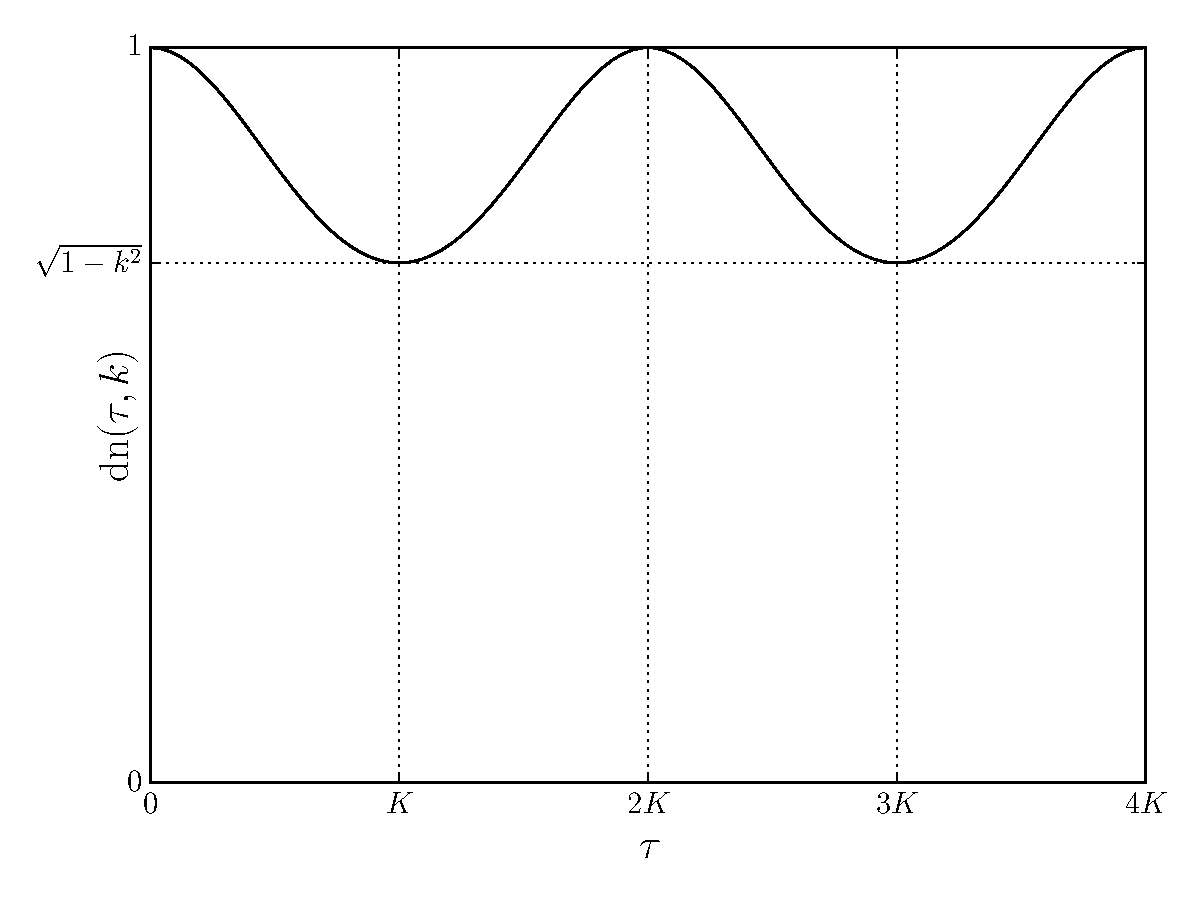
\includegraphics[width=0.5\textwidth]{img/dn_tau_k2}
    \caption{Illustration of the elliptic function $\dn(\tau, k)$.}
    \label{fig: dn tau}
\end{figure}
We can write the periodicity in $t$ by referring to equation \eqref{eqn: tau t}
such that the period is:
\begin{equation}
    T = 4K\sqrt{\frac{I_{1}I_{2}I_{3}}{(I_{3}-I_{2})(M^{2} - 2EI_{1})}}
\end{equation}

This period refers to the motion of $\Omega$ is in the body frame: after one period the 
spin-vector returns to its original position. However, the 
axisymmetric body itself will not return to its original position in the
inertial frame as described by \citet{Landau1969}.

\subsubsection{Return to the wobble angle}
In the body frame then, the polar angle is a periodic function of the precessional
phase. It therefore does make sense to define it as a wobble angle
since it is not constant. Nevertheless, we would like to define an averaged 
wobble angle particuarly in the case where the variations from this average are
small. 

As previously mentiond, the magnitude of the variations is governed by the 
size of the parameter $k$. When $k$ is small the variations are small, this 
limit occurs when
\begin{equation}
    |I_{2} - I_{1}| \ll |I_{3} - I_{2}|,
    \label{eqn: I23 limit}
\end{equation}
such the the body is close to biaxial. From \citet{Abramowitz1972} when
$k^{2} \ll 1$ we may use the approximation
\begin{equation}
    \dn(\tau, k) \approx 1 - \frac{1}{2}k^{2} \sin^{2}\tau + \mathcal{O}(k^{4})
\end{equation}

Time averaging over a single period in $\tau$ we have
\begin{align}
    \langle \dn(\tau, k) \rangle \bigg|_{k \ll 1} \approx  \frac{1}{4K}\int_{0}^{4K} 1 - \frac{1}{2}k^{2} \sin^{2}\tau d\tau & =
    \frac{1}{4K}\left[\tau  - \frac{k^{2}}{4}\left(\tau - \sin\tau\cos\tau\right) \right]_{0}^{4K} \\
    & = \left(1 - \frac{k^{2}}{4}\right)
\end{align}
Therefore we can define the averaged polar angle as
\begin{align}
\langle\sin\theta\rangle& \approx \frac{1}{4K}\int_{0}^{4K}\sin\theta d\tau \\
                 & = \sqrt{\frac{I_{3}(1 - 2EI_{1}/M^{2})}{\left(I_{3} - I_{1}\right)}}
                     \left(1 - \frac{k^{2}}{4}\right)
\label{eqn: bar sin theta triaxial}
\end{align}
%Firstly we can check the consistency of this with equation \eqref{eqn: sin theta biaxial}:
%taking the limit in which the triaxial body become biaxial, that is when
%\begin{align}
%    I_{2}  = I_{1} = I_{0} &&& I_{3} = I_{0}(1 + \epsI)
%\end{align}
%then $k^{2} = 0$ and we recover precisely the constant polar angle for the biaxial
%case given in equation \eqref{eqn: sin theta biaxial}.

We can now simplify by setting the right hand side all under a sqaure root. 
Then, since we are already neglecting term of $\mathcal{O}(k^{4})$, we can
expand to give
\begin{equation}
\langle\sin\theta\rangle \approx
    \left(
    \frac{I_{3}}{I_{3}-I_{1}}
    \left(
    \left(1 - \frac{2EI_{1}}{M^{2}}\right) 
    - \frac{1}{2}\left(\frac{2EI_{3}}{M^{2}} -1\right) \frac{I_{2}-I_{1}}{I_{3}-I_{2}}
\right)
\right)^{1/2}
\end{equation}
From equation \eqref{eqn: I23 limit} it is clear the second term is much smaller 
than the first. Hence in the limit of small triaxiality, the average of
$\sin\theta$ tends too the fixed wobble angle in the biaxial body. Therefore
provided equation \eqref{eqn: I23 limit} holds we may still approximate the wobble
angle by \eqref{eqn: sin theta biaxial}. 

\biblio
\end{document}

